\section{Lecture 5: Superscalar Architecture (SSA)}
Computer designed to improve computation on scalars instructions. \\
A scalar is a variable that can hold only one atomic value at a time, e.g., an integer or a real. \\
A scalar architecture processes one data item at a time -- the computers we discussed up till now. \\
Examples of non-scalar variables: \\
-- Arrays -- Vector Processor \\
-- Matrices -- Graphics Processing Unit (GPU) \\
-- Records \\

In a superscalar architecture (SSA), several scalar instructions can be initiated simulaneously and executed independently.

\subsection{Instruction-level parallelism}
Most operations are on scalar quantities, speed up these operations will lead to large performance improvement.

\subsection{Superpipelining}
Divide pipelining stages into different several sub-stages, and hence increase the number of instructions which are handled by the pipeline at the same time. \\
\todo{A picture would be nice here} \\

-- For example by diving each stage into two sub stages, we will be able (in the ideal situation) to perform each stage at twice the stage. \\
-- No duplication of hardware is needed. \\
-- Not all stages can be divided into (equal length) sub stages. \\
-- Hazards more difficult to resolve. \\
-- More complex hardware. \\
-- Interrupt handling and testing will be more complicated. \\

\subsection{Difference between Superpipelined and Superscalar Designs}
The difference is that Superpipeline can perform several instructions in one clock cycle, whereas Superscalar performs several instructions in parallel

\begin{figure}[H]
  \centering
  \scalebox{0.342}{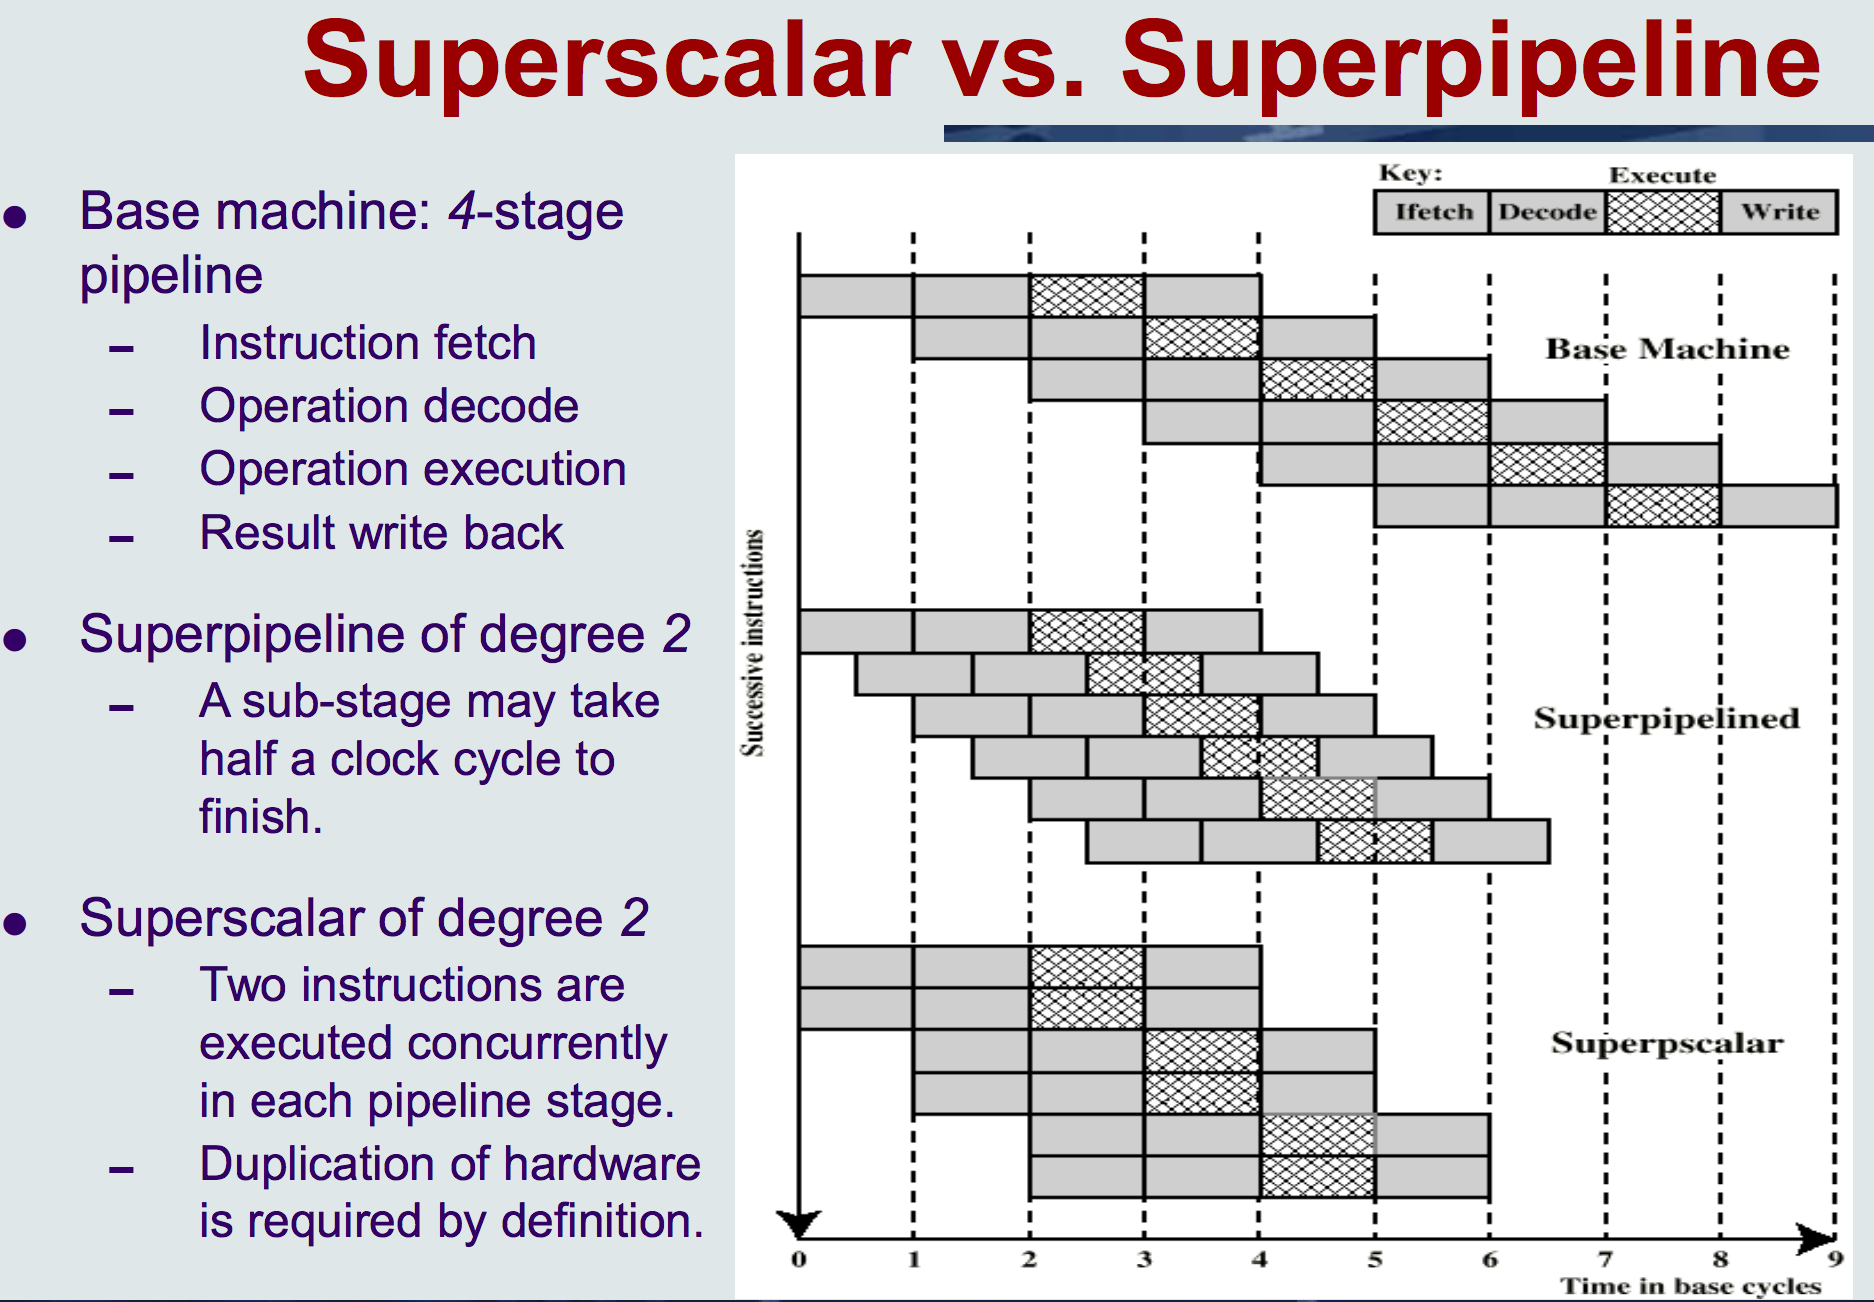
\includegraphics{img/superscalar-vs-superpipeline.png}}
  \caption{Difference between a Superscalar and a Superpipeline architecture}
  \label{fig:superscalar-vs-superpipeline}
\end{figure}


\subsection{Superscalar Superpipeline Design}

\begin{figure}[H]
  \centering
  \scalebox{0.342}{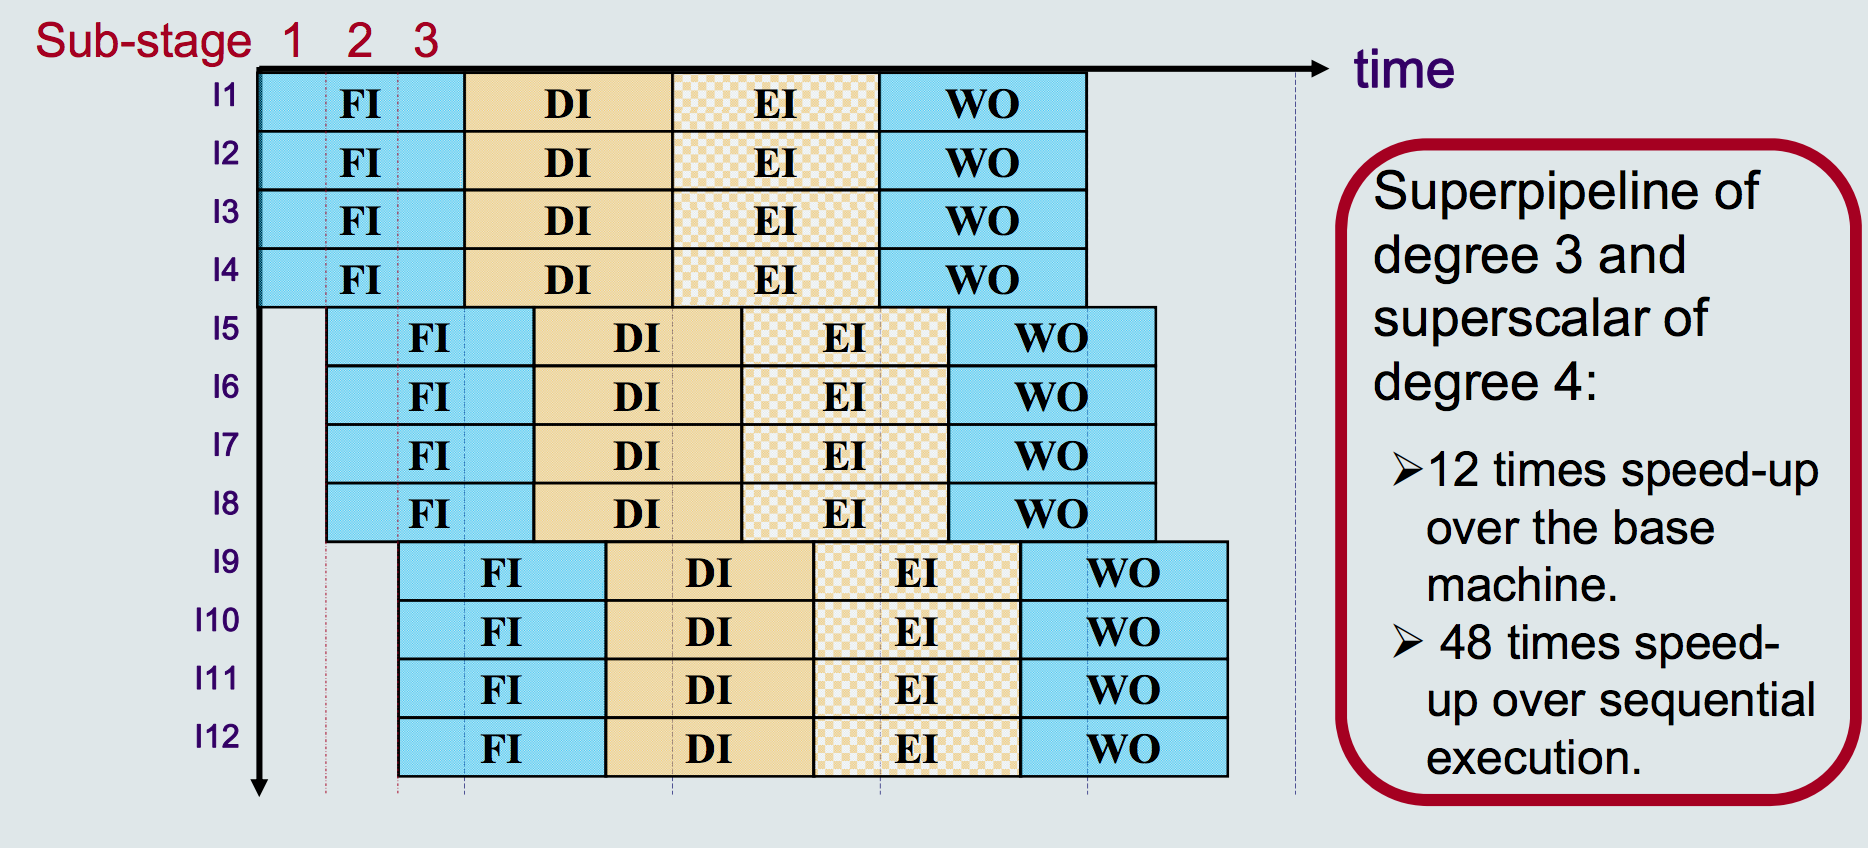
\includegraphics{img/superscalar-superpipeline.png}}
  \caption{Superscalar Superpipeline architecture}
  \label{fig:superscalar-superpipeline}
\end{figure}

The new trend is to combined the two ideas. In Figure \ref{fig:superscalar-superpipeline} it says that this would give us a 48 times speedup, this is not the case though because of data dependencies.

\subsection{Dependency issues}
The main problems are:
-- Resource conflicts. \\
-- Control (procedural) dependency. \\
-- Data dependencies. \\

These are very similar to the cases in normal pipelining (data hazards). But the consequences are more severe here because the parallelism are greater and thus larger amount of performance will be lost. \\

\subsubsection{Resource Conflicts}
Several instructions compete for the same hardware resource at the same time.
-- For instance, two aritmethic instructions need the same floating-point unit for execution. \\
-- similar to structural hazards in pipeline. \\

They can be solved \underline{partly} by introducing several hardware units for the same functions. \\
-- e.g. have two floating point units. \\
-- the hardware units can also be pipelined to support several operations at the same time. \\
-- however, memory units \textbf{can't be duplicated}.

\subsubsection{Procedural Dependency}

\subsubsection{Data Conflicts}

\subsubsection{Window of execution}

\subsubsection{Data Dependency}

\subsubsection{True Data Dependency}

\subsubsection{Output Dependency}

\subsubsection{Anti Dependency}

\subsubsection{Effect of Dependencies}

\subsection{Parallel instruction execution}

\subsubsection{Instruction vs Machine Parallelism}

\subsubsection{Division and Decoupling}

\subsubsection{SSA instruction Execution Policies}

\subsubsection{In-Order with In-Order Completion}
This seems important to understand

\subsubsection{In-Order issue with Out-of-Order Completion}
This seems important to understand
